% Options for packages loaded elsewhere
\PassOptionsToPackage{unicode}{hyperref}
\PassOptionsToPackage{hyphens}{url}
\PassOptionsToPackage{dvipsnames,svgnames,x11names}{xcolor}
%
\documentclass[
  onecolumn]{article}

\usepackage{amsmath,amssymb}
\usepackage{iftex}
\ifPDFTeX
  \usepackage[T1]{fontenc}
  \usepackage[utf8]{inputenc}
  \usepackage{textcomp} % provide euro and other symbols
\else % if luatex or xetex
  \usepackage{unicode-math}
  \defaultfontfeatures{Scale=MatchLowercase}
  \defaultfontfeatures[\rmfamily]{Ligatures=TeX,Scale=1}
\fi
\usepackage{lmodern}
\ifPDFTeX\else  
    % xetex/luatex font selection
\fi
% Use upquote if available, for straight quotes in verbatim environments
\IfFileExists{upquote.sty}{\usepackage{upquote}}{}
\IfFileExists{microtype.sty}{% use microtype if available
  \usepackage[]{microtype}
  \UseMicrotypeSet[protrusion]{basicmath} % disable protrusion for tt fonts
}{}
\makeatletter
\@ifundefined{KOMAClassName}{% if non-KOMA class
  \IfFileExists{parskip.sty}{%
    \usepackage{parskip}
  }{% else
    \setlength{\parindent}{0pt}
    \setlength{\parskip}{6pt plus 2pt minus 1pt}}
}{% if KOMA class
  \KOMAoptions{parskip=half}}
\makeatother
\usepackage{xcolor}
\usepackage[left=35mm,right=35mm,top=15mm,bottom=20mm,noheadfoot]{geometry}
\setlength{\emergencystretch}{3em} % prevent overfull lines
\setcounter{secnumdepth}{-\maxdimen} % remove section numbering
% Make \paragraph and \subparagraph free-standing
\makeatletter
\ifx\paragraph\undefined\else
  \let\oldparagraph\paragraph
  \renewcommand{\paragraph}{
    \@ifstar
      \xxxParagraphStar
      \xxxParagraphNoStar
  }
  \newcommand{\xxxParagraphStar}[1]{\oldparagraph*{#1}\mbox{}}
  \newcommand{\xxxParagraphNoStar}[1]{\oldparagraph{#1}\mbox{}}
\fi
\ifx\subparagraph\undefined\else
  \let\oldsubparagraph\subparagraph
  \renewcommand{\subparagraph}{
    \@ifstar
      \xxxSubParagraphStar
      \xxxSubParagraphNoStar
  }
  \newcommand{\xxxSubParagraphStar}[1]{\oldsubparagraph*{#1}\mbox{}}
  \newcommand{\xxxSubParagraphNoStar}[1]{\oldsubparagraph{#1}\mbox{}}
\fi
\makeatother


\providecommand{\tightlist}{%
  \setlength{\itemsep}{0pt}\setlength{\parskip}{0pt}}\usepackage{longtable,booktabs,array}
\usepackage{calc} % for calculating minipage widths
% Correct order of tables after \paragraph or \subparagraph
\usepackage{etoolbox}
\makeatletter
\patchcmd\longtable{\par}{\if@noskipsec\mbox{}\fi\par}{}{}
\makeatother
% Allow footnotes in longtable head/foot
\IfFileExists{footnotehyper.sty}{\usepackage{footnotehyper}}{\usepackage{footnote}}
\makesavenoteenv{longtable}
\usepackage{graphicx}
\makeatletter
\def\maxwidth{\ifdim\Gin@nat@width>\linewidth\linewidth\else\Gin@nat@width\fi}
\def\maxheight{\ifdim\Gin@nat@height>\textheight\textheight\else\Gin@nat@height\fi}
\makeatother
% Scale images if necessary, so that they will not overflow the page
% margins by default, and it is still possible to overwrite the defaults
% using explicit options in \includegraphics[width, height, ...]{}
\setkeys{Gin}{width=\maxwidth,height=\maxheight,keepaspectratio}
% Set default figure placement to htbp
\makeatletter
\def\fps@figure{htbp}
\makeatother

\usepackage{inputenc}
\usepackage{caption} % Usar el paquete caption para personalizar leyendas
\captionsetup[figure]{name=Figura} % Cambia la palabra "Figure" por "Figura"
\captionsetup[table]{name=Tabela} % Cambia la palabra "Figure" por "Figura"
\makeatletter
\@ifpackageloaded{caption}{}{\usepackage{caption}}
\AtBeginDocument{%
\ifdefined\contentsname
  \renewcommand*\contentsname{Table of contents}
\else
  \newcommand\contentsname{Table of contents}
\fi
\ifdefined\listfigurename
  \renewcommand*\listfigurename{List of Figures}
\else
  \newcommand\listfigurename{List of Figures}
\fi
\ifdefined\listtablename
  \renewcommand*\listtablename{List of Tables}
\else
  \newcommand\listtablename{List of Tables}
\fi
\ifdefined\figurename
  \renewcommand*\figurename{Figure}
\else
  \newcommand\figurename{Figure}
\fi
\ifdefined\tablename
  \renewcommand*\tablename{Table}
\else
  \newcommand\tablename{Table}
\fi
}
\@ifpackageloaded{float}{}{\usepackage{float}}
\floatstyle{ruled}
\@ifundefined{c@chapter}{\newfloat{codelisting}{h}{lop}}{\newfloat{codelisting}{h}{lop}[chapter]}
\floatname{codelisting}{Listing}
\newcommand*\listoflistings{\listof{codelisting}{List of Listings}}
\makeatother
\makeatletter
\makeatother
\makeatletter
\@ifpackageloaded{caption}{}{\usepackage{caption}}
\@ifpackageloaded{subcaption}{}{\usepackage{subcaption}}
\makeatother

\ifLuaTeX
  \usepackage{selnolig}  % disable illegal ligatures
\fi
\usepackage{bookmark}

\IfFileExists{xurl.sty}{\usepackage{xurl}}{} % add URL line breaks if available
\urlstyle{same} % disable monospaced font for URLs
\hypersetup{
  colorlinks=true,
  linkcolor={blue},
  filecolor={Maroon},
  citecolor={Blue},
  urlcolor={Blue},
  pdfcreator={LaTeX via pandoc}}


\author{}
\date{2024-10-31}

\begin{document}


\section{Universidade Federal de
Pernambuco}\label{universidade-federal-de-pernambuco}

\vspace{-.4cm}

\section{Centro de Ciências Exatas e da
Natureza}\label{centro-de-ciuxeancias-exatas-e-da-natureza}

\vspace{-.4cm}

\section{Departamento de
Estatística}\label{departamento-de-estatuxedstica}

\vspace{.5cm}

\subsection{TÓPICOS ESPECIAIS EM ESTATÍSTICA
COMPUTACIONAL}\label{tuxf3picos-especiais-em-estatuxedstica-computacional}

\vspace{.5cm}

\textbf{Data:} 01 de dezembro de 2024

\textbf{Aluno:} Yuri Martí Santana Santos

\vspace{.5cm}

\section{1. Introdução e Visão de
Negócio}\label{introduuxe7uxe3o-e-visuxe3o-de-neguxf3cio}

Este trabalho foca na modelagem preditiva de dados provenientes de
campanhas de marketing direto realizadas por uma instituição bancária
portuguesa, disponibilizados pelo UC Irvine Machine Learning Repository.
Essas campanhas, baseadas em contatos telefônicos, buscavam identificar
a propensão de clientes à subscrição de depósitos a prazo, um produto
estratégico no setor financeiro.

A modelagem preditiva é amplamente utilizada para otimizar campanhas de
marketing, especialmente no setor bancário, devido ao seu impacto na
alocação de recursos e aumento de retornos. Estudos apontam que métodos
baseados em aprendizado de máquina e estatística avançada podem
identificar padrões complexos de comportamento e fornecer subsídios para
a tomada de decisão (Verbraken et al., 2014). Os dados analisados
incluem variáveis demográficas, socioeconômicas e operacionais, como o
histórico de contatos e resultados de campanhas anteriores, permitindo
explorar padrões de comportamento e estratégias de interação (Chen et
al., 2012).

O objetivo principal é desenvolver e comparar modelos para estimar a
probabilidade de subscrição de depósitos, avaliando o desempenho de
diferentes algoritmos preditivos.

\section{2. Conjunto de dados e análise
exploratória}\label{conjunto-de-dados-e-anuxe1lise-exploratuxf3ria}

Os dados utilizados originalmente contêm 41.188 amostras, 20 atributos
(\emph{features}), e estão ordenados de maio de 2008 até novembro de
2010. O conjunto de dados analisado apresenta uma estrutura segmentada,
composta por variáveis que capturam atributos dos clientes,
características das interações realizadas durante as campanhas de
marketing e indicadores contextuais de natureza socioeconômica. Entre os
atributos dos clientes, destacam-se variáveis demográficas e
financeiras, como idade (numérica), ocupação (categórica, com 12
categorias, incluindo ``admin.'' e ``unknown'') e estado civil
(categórica, com categorias como ``married'' e ``unknown'').
Adicionalmente, o nível educacional dos clientes é representado por uma
variável categórica com sete níveis, incluindo ``basic.4y'' e
``university.degree''. Aspectos relacionados à situação financeira são
capturados por variáveis binárias que indicam a existência de crédito em
inadimplência, empréstimos habitacionais e empréstimos pessoais.

As variáveis relacionadas ao contato telefônico refletem a dinâmica
operacional das campanhas. O tipo de comunicação utilizada é
representado pela variável \emph{contact} (categórica: ``cellular'' ou
``telephone''), enquanto as variáveis mês e dia da semana do último
contato fornecem informações temporais. A variável duração, embora
informativa para fins de \emph{benchmark}, deve ser tratada com cautela,
pois seu valor é conhecido apenas após a realização da chamada. Outras
variáveis importantes incluem o número total de contatos realizados na
campanha atual (\emph{campaign}), a quantidade de dias desde o último
contato em campanhas anteriores (\emph{pdays}) e o resultado da última
campanha (\emph{poutcome}), que podem indicar padrões históricos de
interação. Por fim, variáveis macroeconômicas, como a taxa de variação
de emprego (\emph{emp.var.rate}) e o índice Euribor de três meses
(\emph{euribor3m}), oferecem contexto sobre o ambiente econômico em que
as campanhas foram realizadas, enriquecendo a análise preditiva com
informações contextuais relevantes.

A campanha atual contou com uma taxa de sucesso de 11\%, em contraste
com a campanha anterior, que obteve uma taxa de sucesso de apenas 3\%.
Contudo, independentemente da campanha realizada, os valores indicam uma
sub-representação, na amostra, daqueles que realizam o objetivo de
subscrever um depósito. Essa disparidade é exemplificada na Figura 1.

\begin{figure}[H]

{\centering 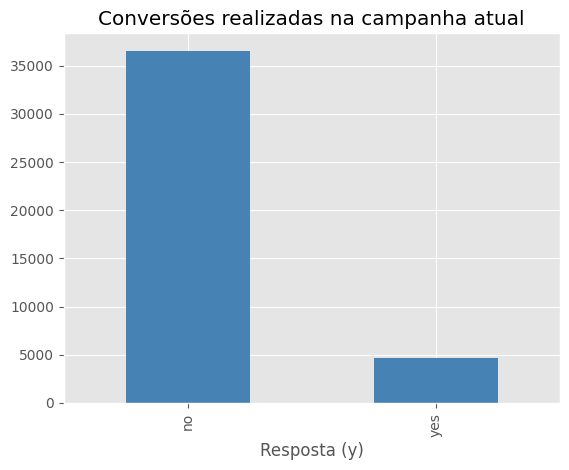
\includegraphics[width=0.5\textwidth,height=\textheight]{hist_y.png}

}

\caption{Conversões realizadas com sucesso (\emph{yes}) ou fracasso
(\emph{no}) na campanha atual}

\end{figure}%

A análise exploratória das variáveis identificou uma baixa
representatividade de ocupações consideradas ``não tradicionais'', o que
pode justificar sua agregação para simplificação analítica. O banco
demonstra um mapeamento detalhado do estado civil dos clientes e
registra uma incidência negligenciável de indivíduos analfabetos,
sugerindo um nível educacional elevado entre os clientes. A ocorrência
de inadimplência é igualmente rara, refletindo critérios rigorosos na
seleção de clientes elegíveis para ofertas financeiras. Observou-se uma
proporção equilibrada de clientes com e sem empréstimos habitacionais,
enquanto empréstimos pessoais são significativamente menos frequentes.
Em relação às estratégias de comunicação, quase o dobro das interações
foi realizado por celular em comparação ao telefone fixo, e houve uma
redução no número de chamadas na segunda metade do ano, possivelmente
associada a padrões sazonais. Além disso, as chamadas estão
uniformemente distribuídas ao longo dos dias úteis. Os dados também
revelam uma segmentação clara entre clientes previamente contatados e
aqueles que nunca foram abordados, evidenciando distintos níveis de
engajamento e interação com o banco, conforme ilustrado na Figura 2.

\begin{figure}[H]

{\centering 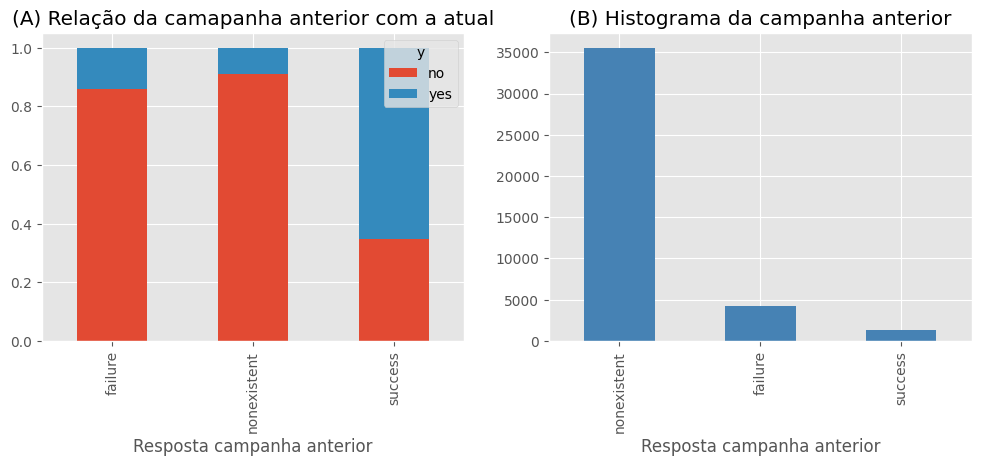
\includegraphics[width=1\textwidth,height=\textheight]{hist_pout.png}

}

\caption{(A) Demonstra a reincidência daqueles que tiveram no passado,
mas (B) não apresenta um volume significativo de reincidentes}

\end{figure}%

\section{3. Metodologia e fundamentos
teóricos}\label{metodologia-e-fundamentos-teuxf3ricos}

As seções anteriores foram dedicadas ao processo de entendimento do
negócio (Seção 1) e dos dados (Seção 2). Agora, será detalhado quais
métodos e princípios guiam o pré-processamento dos dados, as modelagens
escolhidas, como redes totalmente conectadas, e o ambiente
computacional.

\subsubsection{Métodos de Pré-Processamento de
Dados}\label{muxe9todos-de-pruxe9-processamento-de-dados}

O pré-processamento visa aprimorar a qualidade dos dados para os
modelos, minimizando vieses e inconsistências. Os métodos utilizados
incluem balanceamento de dados, tratamento de variáveis com baixa
ocorrência e \emph{leaky}, transformação de variáveis categóricas e
numéricas.

\begin{itemize}
\tightlist
\item
  \textbf{Balanceamento de classes}: Ajusta a distribuição das classes
  no conjunto de treinamento, utilizando subamostragem ou
  superamostragem para reduzir o viés de distribuições desiguais;
\item
  \textbf{One-hot encoding}: Transformação de uma variável categórica em
  diversas variáveis binárias;
\item
  \textbf{Remoção de variáveis com baixa ocorrência de rótulos}: Exclui
  variáveis que geral problemas na transformação de variáveis via
  \emph{one-hot encoding}, em razão da baixa frequência de certos
  rótulos que prejudiza o processo de amostrada pelo raro-efeito da
  existência do atributo;
\item
  \textbf{Exclusão de variáveis \emph{leaky}}: Remove variáveis cujos
  valores dependem de informações disponíveis após a predição, evitando
  distorções no modelo;
\item
  \textbf{Normalização de variáveis numéricas}: Ajusta as variáveis para
  uma escala uniforme, garantindo que todas as variáveis tenham o mesmo
  peso no modelo.
\end{itemize}

\subsection{Redes totalmente
conectadas}\label{redes-totalmente-conectadas}

Uma rede neural totalmente conectada é uma arquitetura na qual cada
neurônio em uma camada está conectado a todos os neurônios da camada
subsequente. Essa estrutura é utilizada devido à sua capacidade de
modelar relações complexas entre variáveis de entrada e saída. Cada
conexão é ponderada e ajustada durante o treinamento para minimizar uma
função de perda, permitindo à rede aprender padrões nos dados.

O processamento de uma camada é representado por:

\[\mathbf{y} = f(\mathbf{W} \cdot \mathbf{x} + \mathbf{b}),\]

onde \(\mathbf{x}\) é o vetor de entrada, \(\mathbf{W}\) é a matriz de
pesos, \(\mathbf{b}\) é o vetor de viés e \(f(\cdot)\) é a função de
ativação.

\subsubsection{Funções de
ativação}\label{funuxe7uxf5es-de-ativauxe7uxe3o}

\begin{itemize}
\item
  \textbf{Função de ativação ReLU (Rectified Linear Unit):} uma função
  não linear que retorna o valor da entrada quando este é positivo e
  zero quando é negativo.
\item
  \textbf{Função de ativação sigmoid:} uma função logística que mapeia
  qualquer valor de entrada para um intervalo entre 0 e 1. É
  particularmente útil em problemas de classificação binária, pois
  introduz não linearidades e ajuda a modelar probabilidades, embora
  possa sofrer com o problema de gradientes saturados em valores
  extremos de entrada.
\end{itemize}

\subsubsection{Dropout}\label{dropout}

O dropout é uma técnica utilizada em redes neurais para reduzir o risco
de sobreajuste durante o treinamento. Consiste em desativar
aleatoriamente uma porcentagem de unidades (perceptrons) de cada camada
da rede em cada iteração, forçando a rede a aprender representações mais
robustas e generalizáveis dos dados. Durante o treinamento, a
probabilidade de desativação de cada perceptron é definida por um
parâmetro chamado taxa de dropout, que varia entre 0 e 1.

\subsection{Ambiente computacional}\label{ambiente-computacional}

O ambiente computacional no qual as atividades foram desenvolvidas foi o
Google Colab, uma plataforma em nuvem oferecida pelo Google que executa
código Python em notebooks interativos.

Neste contexto, destaca-se o uso da biblioteca Keras para modelagem.
Trata-se de uma API de alto nível para construção e treinamento de redes
neurais, que integra o TensorFlow, um dos frameworks de aprendizado
profundo mais amplamente utilizados.

\section{4. Modelagem}\label{modelagem}

\subsection{Pré-processamento}\label{pruxe9-processamento}

Devido à sub-representação das variáveis-resposta, foram criadas duas
amostras de treinamento: uma com 80\% dos dados, denominada
\emph{Amostra A}, e outra, de tamanho fixo (8.382 observações),
balanceada com igual número de ocorrências de conversões bem-sucedidas e
mal-sucedidas, denominada \emph{Amostra B}.

A variável de inadimplência foi removida devido ao seu baixo número de
ocorrências, o que dificultava a correta segmentação das amostras.
Adicionalmente, a variável de duração da ligação foi excluída por ser
considerada uma variável \emph{leaky}, ou seja, que não estaria
disponível no momento da predição, uma vez que seu valor é conhecido
apenas após o término da interação.

As variáveis foram separadas em categóricas e numéricas para o
tratamento adequado. As variáveis categóricas passaram por um processo
de \emph{one-hot encoding}, com a exclusão de pelo menos um rótulo para
evitar a armadilha das variáveis \emph{dummy}. As variáveis numéricas
foram normalizadas para garantir compatibilidade com os modelos.

\subsection{Modelos e treinamento}\label{modelos-e-treinamento}

Após o pré-processamento, foram avaliados cinco modelos distintos. O
Modelo 0 busca replicar uma regressão logística como \emph{baseline}. A
partir deste, foram desenvolvidos os demais modelos, conforme descrito
na Tabela 1. Na coluna ``Estrutura'', é detalhada a quantidade de
perceptrons em cada camada, representada pelo tamanho do vetor, sendo o
número de elementos equivalente à quantidade de camadas (incluindo as
camadas de entrada e saída). A coluna ``Função de Ativação'' especifica
as funções utilizadas em cada camada, onde \emph{I} representa a camada
inicial, \emph{S} indica o uso de uma função de ativação sigmoid e
\emph{R} refere-se ao uso de uma função de ativação ReLU. Por fim, a
coluna ``Dropout'' informa os valores de dropout aplicados a cada
camada.

\begin{longtable}[]{@{}
  >{\centering\arraybackslash}p{(\columnwidth - 8\tabcolsep) * \real{0.1176}}
  >{\centering\arraybackslash}p{(\columnwidth - 8\tabcolsep) * \real{0.2118}}
  >{\raggedright\arraybackslash}p{(\columnwidth - 8\tabcolsep) * \real{0.2000}}
  >{\raggedright\arraybackslash}p{(\columnwidth - 8\tabcolsep) * \real{0.2353}}
  >{\raggedright\arraybackslash}p{(\columnwidth - 8\tabcolsep) * \real{0.2353}}@{}}
\caption{Modelos treinados}\tabularnewline
\toprule\noalign{}
\begin{minipage}[b]{\linewidth}\centering
Modelo
\end{minipage} & \begin{minipage}[b]{\linewidth}\centering
Dados de treino
\end{minipage} & \begin{minipage}[b]{\linewidth}\raggedright
Estrutura
\end{minipage} & \begin{minipage}[b]{\linewidth}\raggedright
Função de Ativação
\end{minipage} & \begin{minipage}[b]{\linewidth}\raggedright
Dropout
\end{minipage} \\
\midrule\noalign{}
\endfirsthead
\toprule\noalign{}
\begin{minipage}[b]{\linewidth}\centering
Modelo
\end{minipage} & \begin{minipage}[b]{\linewidth}\centering
Dados de treino
\end{minipage} & \begin{minipage}[b]{\linewidth}\raggedright
Estrutura
\end{minipage} & \begin{minipage}[b]{\linewidth}\raggedright
Função de Ativação
\end{minipage} & \begin{minipage}[b]{\linewidth}\raggedright
Dropout
\end{minipage} \\
\midrule\noalign{}
\endhead
\bottomrule\noalign{}
\endlastfoot
Modelo 0 & Amostra A & (49, 1) & (I, S) & (0, 0) \\
Modelo 1 & Amostra B & (49, 40, 32, 1) & (I, S, S, S) & (0, 0, 0, 0) \\
Modelo 2 & Amostra A & (49, 49, 49, 1) & (I, S, S, S) & (0, 0.25, 0.25,
0) \\
Modelo 3 & Amostra B & (49, 40, 32, 1) & (I, S, S, S) & (0.2, 0.2, 0,
0) \\
Modelo 4 & Amostra B & (49, 40, 32, 1) & (I, R, R, S) & (0.2, 0.2, 0,
0) \\
\end{longtable}

Os treinamentos foram realizados utilizando coortes de 20\% dos dados
para validação. O Modelo 0 e o Modelo 1 foram treinados por 25 épocas,
enquanto os Modelos 2, 3 e 4 foram treinados por 75 épocas, de modo a
otimizar o aprendizado e avaliar o impacto de diferentes configurações
de estrutura e hiperparâmetros.

\section{5. Avaliação dos
Resultados}\label{avaliauxe7uxe3o-dos-resultados}

A avaliação dos modelos foi realizada com base nos dados de teste,
conforme apresentado na Tabela 2. Nesse contexto, o Modelo 2 demonstrou
o melhor desempenho, alcançando uma acurácia de 0,901 e uma perda de
0,273. Esses resultados indicam uma combinação eficaz de alta precisão e
baixo erro. O Modelo 0 (Regressão Logística) apresentou uma acurácia
igualmente elevada (0,900), mas com uma perda ligeiramente maior
(0,278), sugerindo um desempenho muito próximo ao do Modelo 2, embora
com uma estrutura consideravelmente mais simples e menos parâmetros.

O Modelo 1 exibiu o pior desempenho, com acurácia de 0,580 e perda de
0,848, evidenciando uma significativa discrepância entre as previsões e
os valores reais, o que aponta para um aprendizado ineficiente. Já os
Modelos 3 (acurácia de 0,695, perda de 0,768) e 4 (acurácia de 0,692,
perda de 0,755) apresentaram desempenho intermediário, com uma taxa de
acerto moderada, mas perdas relativamente elevadas. Isso sugere que,
apesar de um desempenho razoável, esses modelos podem enfrentar desafios
na generalização para novos dados.

\begin{longtable}[]{@{}ccc@{}}
\caption{Métricas de avaliação com dados de teste}\tabularnewline
\toprule\noalign{}
Modelo & Acurácia & Perda (\emph{Loss}) \\
\midrule\noalign{}
\endfirsthead
\toprule\noalign{}
Modelo & Acurácia & Perda (\emph{Loss}) \\
\midrule\noalign{}
\endhead
\bottomrule\noalign{}
\endlastfoot
Modelo 0 & 0,900 & 0,278 \\
Modelo 1 & 0,580 & 0,848 \\
Modelo 2 & 0,901 & 0,273 \\
Modelo 3 & 0,695 & 0,768 \\
Modelo 4 & 0,692 & 0,755 \\
\end{longtable}

É importante destacar que o Modelo 1 se diferencia do Modelo 3 apenas
pela aplicação da técnica de \emph{dropout} em determinadas camadas da
rede.

Adicionalmente, as altas acurácias observadas nos Modelos 0 e 2 podem
ser atribuídas, em grande parte, à representação desproporcional dos
dados de não conversão em relação aos de conversão de depósitos. Essa
característica é evidenciada pelas matrizes de confusão dos modelos,
conforme ilustrado na Figura 3.

\begin{figure}[H]

{\centering 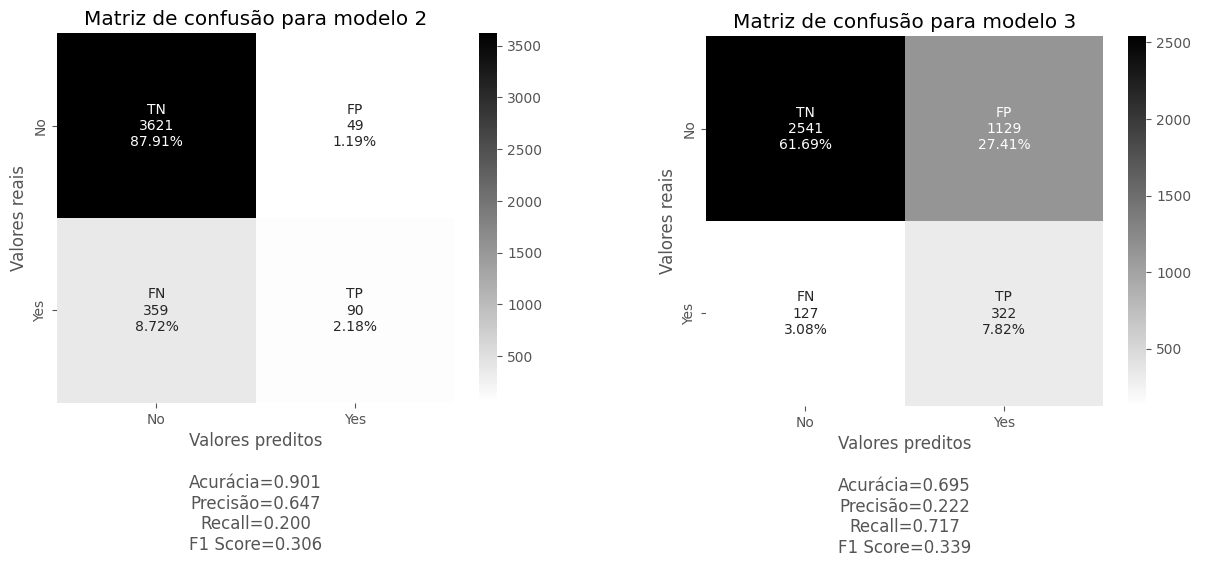
\includegraphics[width=1.1\textwidth,height=\textheight]{cf_matrix.png}

}

\caption{Matrizes de confusão do Modelo 2 e Modelo 3, acompanhadas de
outras métricas}

\end{figure}%

Considerando a finalidade prática dos modelos, os Modelos 3 e 4
mostram-se mais adequados, uma vez que, dentro dos valores previstos
como verdadeiros, apresentam melhores ajustes e precisão. Esses modelos
são capazes de lidar melhor com a classificação positiva, o que é
essencial para otimizar as decisões de negócio no contexto analisado.

\newpage

\section{6. Considerações Finais}\label{considerauxe7uxf5es-finais}

Este trabalho reforça a relevância de técnicas de pré-processamento,
como o balanceamento de classes, no contexto de classificação binária.
Ademais, observou-se o impacto positivo do uso da técnica de
\emph{dropout} nos modelos ensaiados, evidenciado pelo aumento da
acurácia do Modelo 1 (58\%) para 70\% no Modelo 3. Ressalta-se que a
avaliação de modelos deve considerar o contexto da aplicação, onde
métricas como \emph{recall} podem ter maior relevância que a acurácia,
tornando os Modelos 3 e 4 mais adequados para o problema em questão.

Embora este estudo tenha explorado pontos cruciais, há necessidade de
discussões mais amplas sobre enriquecimento de dados e análise de
causalidade, conforme abordado em Moro et al.~(2011). Futuras pesquisas
poderiam explorar novos modelos focados exclusivamente na otimização do
\emph{recall} e incorporar métodos automáticos para ajuste de
hiperparâmetros, visando identificar arquiteturas de rede mais robustas.

Agradecimentos especiais são direcionados ao material disponibilizado no
site da disciplina de Tópicos Especiais em Estatística Computacional
(Ferreira, 2024), que forneceu fundamentos para os scripts e análises
desenvolvidos neste trabalho.

\section{Disclaimer}\label{disclaimer}

Este ensaio buscou sintetizar os principais aspectos de análise viáveis
para um \emph{short paper} de até seis páginas. O processo completo de
construção dos modelos e escolha dos hiperparâmetros reflete um esforço
mais abrangente de exploração, que não pode ser totalmente documentado
neste formato. Em particular, aspectos como correlação e outras métricas
que impactam diretamente o espaço de atributos (\emph{feature space})
não foram detalhados, mas são reconhecidos como relevantes para qualquer
análise.

\section{Referências}\label{referuxeancias}

Chen, H., Chiang, R. H., \& Storey, V. C. (2012). Business intelligence
and analytics: From big data to big impact. MIS quarterly, 1165-1188.

Ferreira, J. A.. Tópicos Especiais em Estatística Computacional. (2024,
Dezembro). UFPE.
https://www.de.ufpe.br/\textasciitilde jodavid/material/topicos\_especiais\_est\_compu/pagina/\_site/

Moro, S., Laureano, R., \& Cortez, P. (2011). Using data mining for bank
direct marketing: An application of the crisp-dm methodology. In
Proceedings of the European Simulation and Modelling Conference-ESM
(Vol. 2011).

Moro, S., Rita, P., \& Cortez, P. (2014). Bank Marketing {[}Dataset{]}.
UCI Machine Learning Repository. https://doi.org/10.24432/C5K306.

Verbraken, T., Verbeke, W., \& Baesens, B. (2014). Profit optimizing
customer churn prediction with Bayesian network classifiers. Intelligent
Data Analysis, 18(1), 3-24.




\end{document}
